% !TEX TS-program = pdflatex
% !TEX encoding = UTF-8 Unicode

% This is a simple template for a LaTeX document using the "article" class.
% See "book", "report", "letter" for other types of document.

\documentclass[11pt]{article} % use larger type; default would be 10pt

\usepackage[utf8]{inputenc} % set input encoding (not needed with XeLaTeX)

%%% Examples of Article customizations
% These packages are optional, depending whether you want the features they provide.
% See the LaTeX Companion or other references for full information.

%%% PAGE DIMENSIONS
\usepackage{geometry} % to change the page dimensions
\geometry{a4paper} % or letterpaper (US) or a5paper or....
% \geometry{margin=2in} % for example, change the margins to 2 inches all round
% \geometry{landscape} % set up the page for landscape
%   read geometry.pdf for detailed page layout information

\usepackage{graphicx} % support the \includegraphics command and options

% \usepackage[parfill]{parskip} % Activate to begin paragraphs with an empty line rather than an indent

%%% PACKAGES
\usepackage{booktabs} % for much better looking tables
\usepackage{array} % for better arrays (eg matrices) in maths
\usepackage{paralist} % very flexible & customisable lists (eg. enumerate/itemize, etc.)
\usepackage{verbatim} % adds environment for commenting out blocks of text & for better verbatim
\usepackage{subfig} % make it possible to include more than one captioned figure/table in a single float
% These packages are all incorporated in the memoir class to one degree or another...
\graphicspath{ {images/} }
\usepackage{floatrow}

\usepackage{listings}

%%% HEADERS & FOOTERS
\usepackage{fancyhdr} % This should be set AFTER setting up the page geometry
\pagestyle{fancy} % options: empty , plain , fancy
\renewcommand{\headrulewidth}{0pt} % customise the layout...
\lhead{}\chead{}\rhead{}
\lfoot{}\cfoot{\thepage}\rfoot{}
\usepackage{listings}


%%% SECTION TITLE APPEARANCE
\usepackage{sectsty}
\allsectionsfont{\sffamily\mdseries\upshape} % (See the fntguide.pdf for font help)
% (This matches ConTeXt defaults)

%%% ToC (table of contents) APPEARANCE
\usepackage[nottoc,notlof,notlot]{tocbibind} % Put the bibliography in the ToC
\usepackage[titles,subfigure]{tocloft} % Alter the style of the Table of Contents
\renewcommand{\cftsecfont}{\rmfamily\mdseries\upshape}
\renewcommand{\cftsecpagefont}{\rmfamily\mdseries\upshape} % No bold!

%%% END Article customizations

%%% The "real" document content comes below...

\title{CS 770: Assignment 5}
\author{Ronghao Yang\\ID: 20511820}
%\date{} % Activate to display a given date or no date (if empty),
         % otherwise the current date is printed 

\begin{document}
\maketitle

\section{Exercise 1}
\begin{lstlisting}[language=Octave, basicstyle=\ttfamily]
function [C,A] = myDFT(f,X)
% discrete Fourier transform
% Output: C,A
% C contains the DFT coefficients
% A contains the DFT approxmiation
% Input: f,X
% f contains the function values
% X contains the X values which are to be approximated
    
    n = length(f);
    % n is the number of points
    
    C=zeros(1,n);
    % initialize the coefficients to 0
    
    i = sqrt(-1);
    % initialize i
    
    for k = 0:n-1
        for j = 0:n-1
            C(k+1) = C(k+1)+(1./n)*f(j+1)*exp(-2*pi*k*(j./n)*i);
        end
    end
    % Calculating the DFT coefficients
    
    N = length(X);
    A = zeros(1,N);
    
    for i = 1:N
        for j = 1:(n-1)./2
            A(i) = A(i) + 2*real(C(j+1))*cos(2*pi*j*X(i))-...
            2*imag(C(j+1))*sin(2*pi*j*X(i));
        end
        A(i) = A(i) + C(1);
    end
    % Calculating the DFT approximations
end
\end{lstlisting}
Note: this function only works with odd number of sampling points, for question 2, we have only tested it on odd number of sapling points.\\
\section{Exercise 2}
\subsection{Exercise 2a}
$f(x)=x$, When n = 101\\
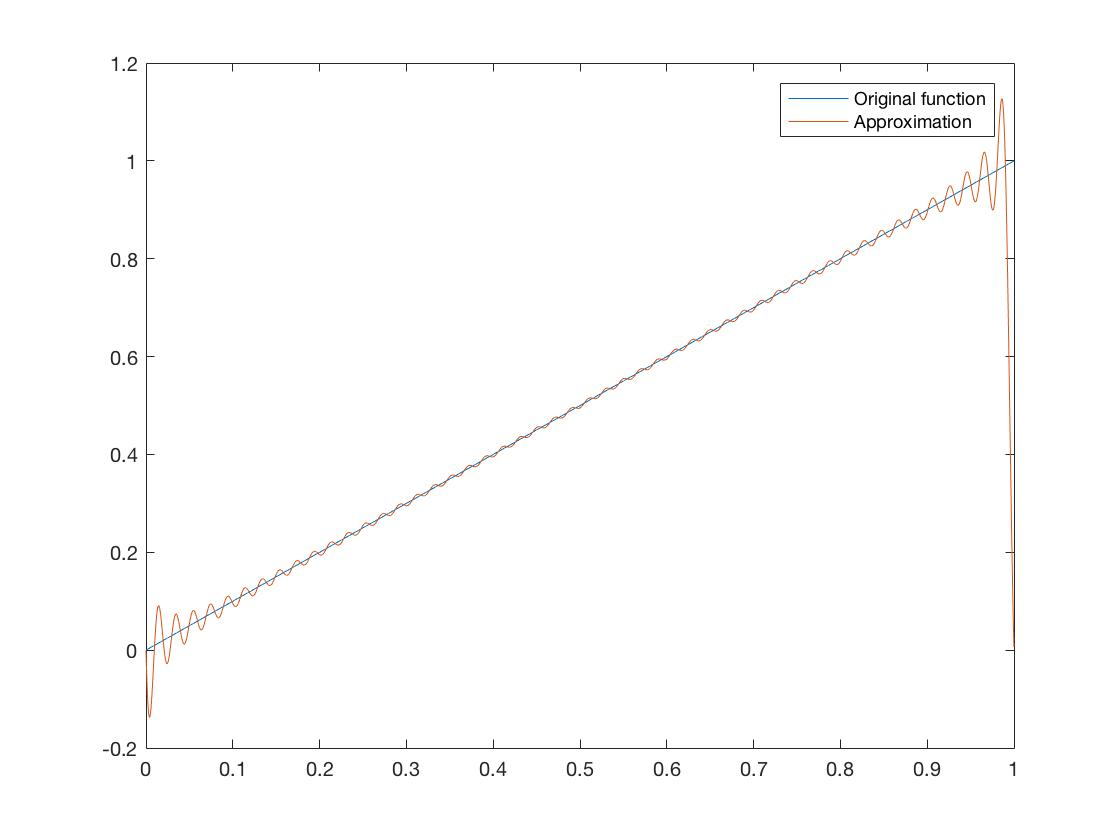
\includegraphics[scale=0.3]{e211.jpg}\\
As we can see here, there is oscillation near the discontinuity of the function.
\subsection{Exercise 2b}
$f(x)=exp(cos(2\pi x))$, When n = 21\\
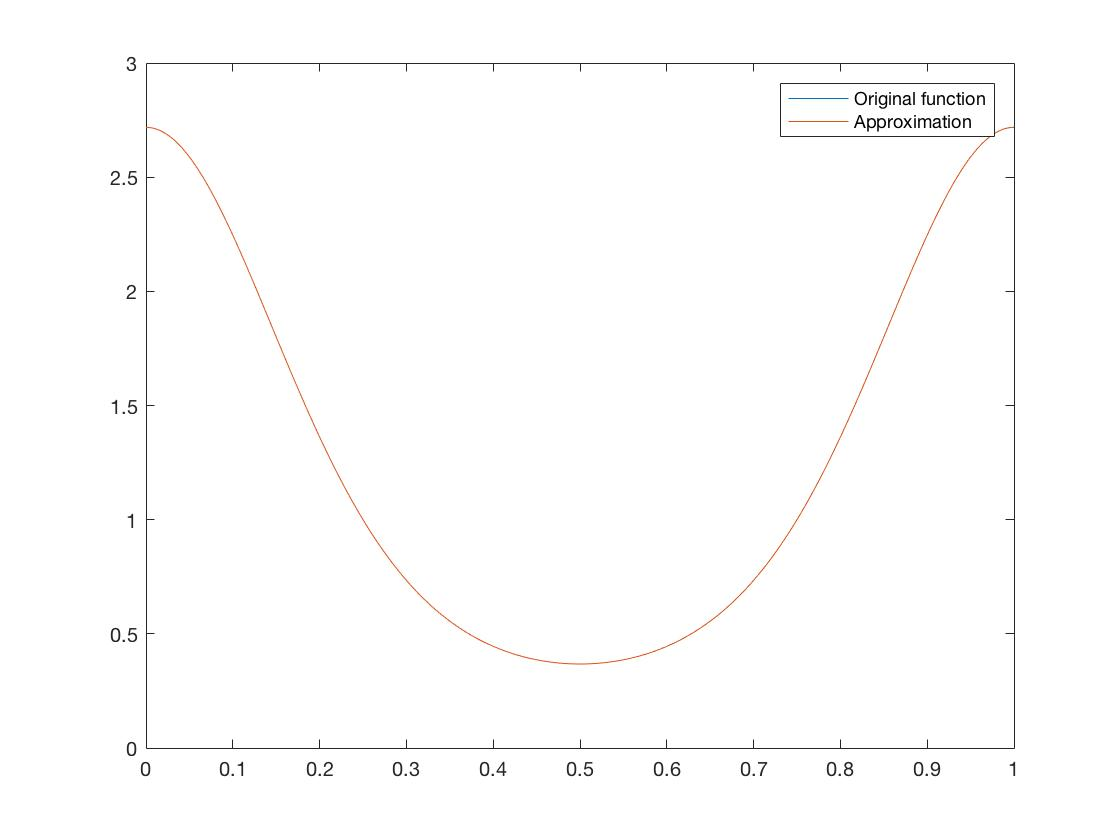
\includegraphics[scale=0.3]{e221.jpg}\\
We have a good approximation here.
\subsection{Exercise 2c}
$f(x)=((x-0.5)/0.5)^{2}$, When n = 21\\
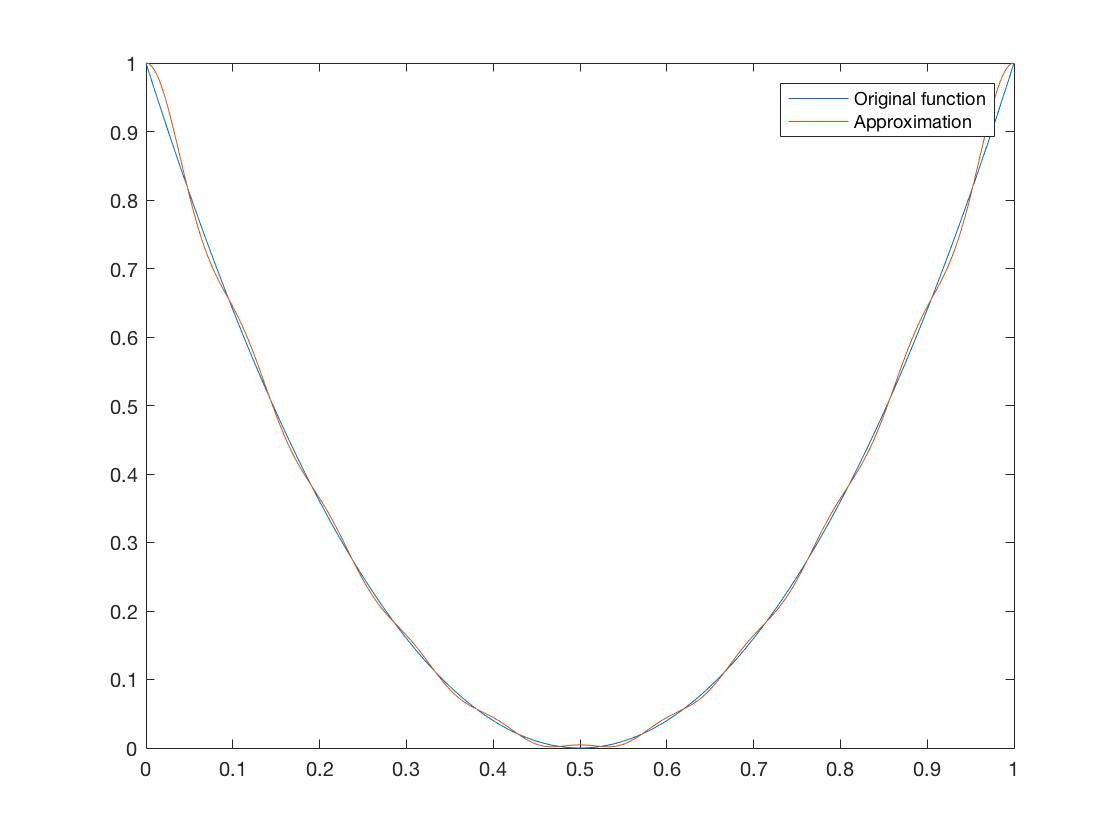
\includegraphics[scale=0.3]{e231.jpg}\\
As we can see here, the approximation here is not as good as (b), the reason is that although the function is continuous, however it's not differentiable at boundary points. Therefore 
\subsection{Exercise 2d}
$f(x)=((x-0.5)/0.5)^{m}$, For this question we set n to be 21\\
When m = 5:\\
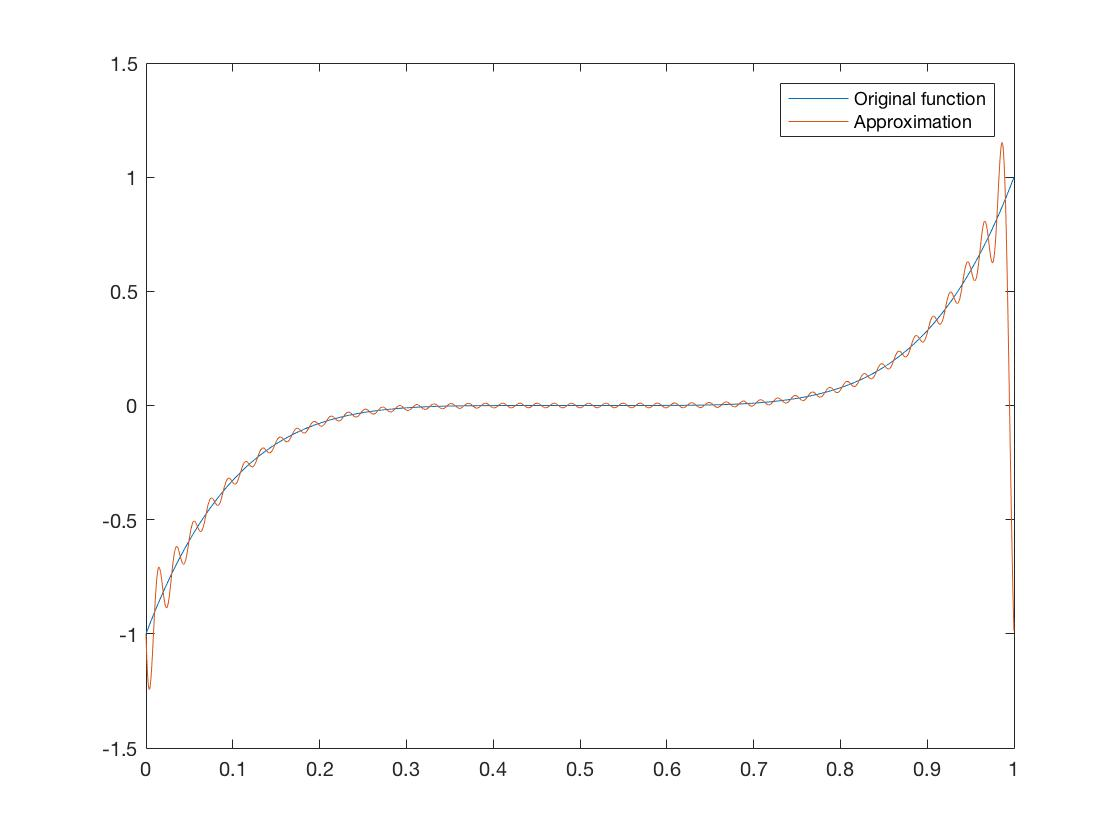
\includegraphics[scale=0.3]{e241.jpg}\\
When m = 10:\\
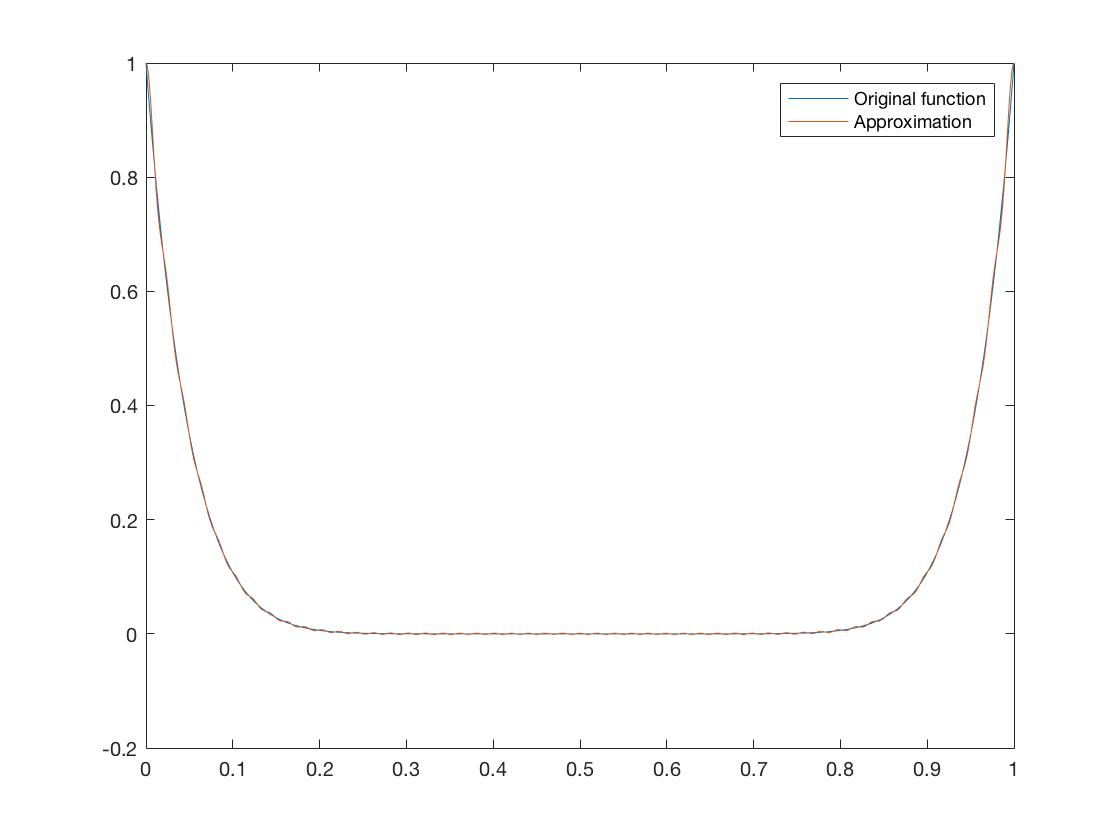
\includegraphics[scale=0.3]{e242.jpg}\\
When m = 25:\\
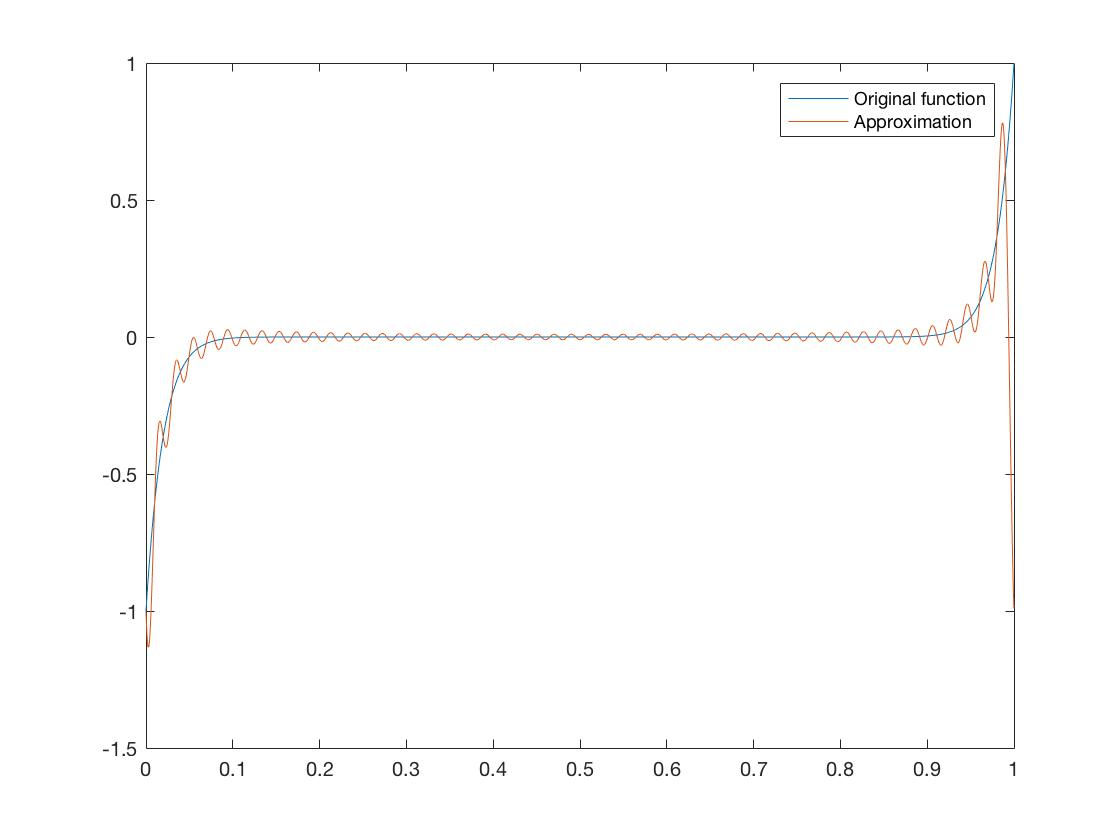
\includegraphics[scale=0.3]{e243.jpg}\\
When m = 50:\\
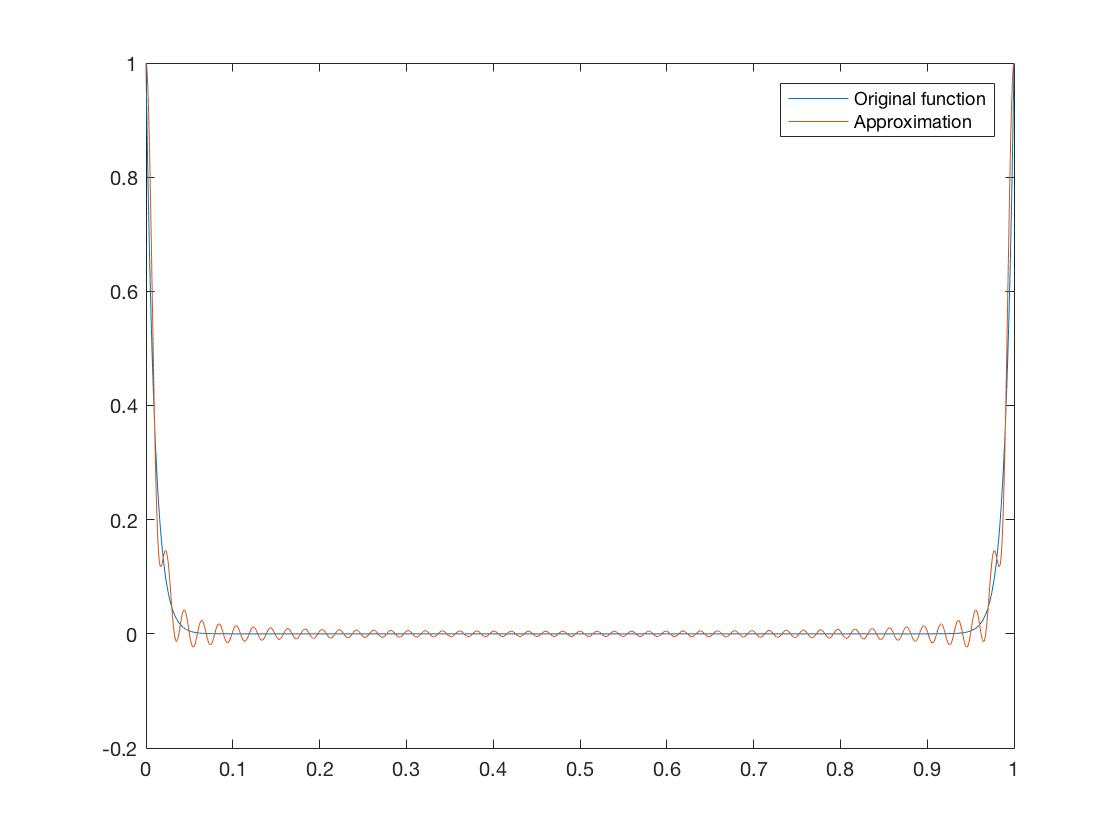
\includegraphics[scale=0.3]{e244.jpg}\\
When m is odd, function f is an odd function on the interval, therefore, f is non-differentiable and discontinuous. Compared to an even m, the Fourier approximation is worse for odd functions.\\\\
Moreover, when m increases, the function at boundary points become steeper and steeper, the absolute value of the derivatives becomes higher and higher, function becomes less and less differentiable. Therefore, as m increases, the Fourier approximation becomes worse and worse.

\section{Exercise 3}
For Fourier series,\\\\
\centerline{$a_{k}$ = $2\int_{0}^{1}f(x)cos(2\pi k x)dx$, $b_{k}$ = $2\int_{0}^{1}f(x)sin(2\pi k x)dx$}
\subsection{Exercise 3a}
For $f(x)=(cos(8\pi x))^{4}$, \\\\
\centerline{$a_{k}$ = $2\int_{0}^{1}(cos(8\pi x))^{4}cos(2\pi k x)dx$, $b_{k}$ = $2\int_{0}^{1}(cos(8\pi x))^{4}sin(2\pi k x)dx$}\\\\
\centerline{Since $cos(2x) = 2cos(x)^{2}-1$}\\\\
\centerline{Then $cos(8\pi x)^{4}$ = $\frac{1}{4}(\frac{cos(32\pi x)}{2}+2cos(16\pi x)+1)$}\\\\
By the orthogonality property,\\\\
\centerline{$a_{0} = \frac{3}{8}$, $a_{8} = \frac{1}{2}$, $a_{16} = \frac{1}{8}$, All $b_{k}$ is 0}\\\\
Then the continuous Fourier series is\\\\
\centerline{$f(x)$ = $\frac{3}{8} + \frac{1}{2}cos(16\pi x)+\frac{1}{8}cos(32\pi x)$}\\\\
For discrete Fourier coefficients, when n = 5:\\\\
\centerline{$a_{0} = C_{0}$}\\\\
when n = 11:\\\\
\centerline{$a_{0} = C_{0},$}\\\\
when n = 21:\\\\
\centerline{$a_{0} = C_{0}, a_{8} = 2\times Real(C_{8})$}\\\\
We expect $a_{k} = 2\times Real(C_{k}), b_{k} = 2\times Imag(C_{k})$ up to n/2, and all other $C_{k}$s to have 0 real parts and 0 imaginary parts. However, this is not the case when we don't have enough sampling points. The coefficients of some high frequency terms also show up in the $C_{k}s$, this is because of aliasing. For example, when n = 11.\\\\
\centerline{$C_{5} = 0.0625$}\\\\
 -$2\times C_{5}$ equals the coefficient of $cos(32\pi x)$. If we compared between $cos(32\pi x)$ and $cos(10\pi x)$, they give the same values at the sampling points. Similar phenomenons also show up when n equals other values.
\subsection{Exercise 3b}
For $f(x)=x$,\\\\
%\centerline{$C_{k}$ = $\int_{0}^{1}xe^{-2\pi i k x}$}\\\\
%\centerline{Let $u = x, \frac{dv}{dx} = e^{-2\pi i k x}$}\\\\
%\centerline{Then $du = 1, v = \frac{1}{-2\pi i k}e^{-2\pi i k x}$}\\\\
%\centerline{Then $\int xe^{-2\pi i k x}$  = $\frac{x}{-2\pi i k}e^{-2\pi i k x}-\int \frac{1}{-2\pi i k}e^{-2\pi i k x}$}\\\\
%\centerline{$\int xe^{-2\pi i k x}$ = $\frac{x}{-2\pi i k}e^{-2\pi i k x}-\frac{1}{-4\pi^{2}k^2}e^{-2\pi i k x}$}\\\\
%\centerline{Since $C_{k}$ = $\int_{0}^{1}xe^{-2\pi i k x}$}\\\\
%\centerline{Then $C_{k}$ = $(\frac{1}{-2\pi i k}e^{-2\pi i k}-\frac{1}{-4\pi^{2}k^2}e^{-2\pi i k}) - (0 - \frac{1}{-4\pi^{2}k^2})$}\\\\
%\centerline{$C_{k}$ = $\frac{•}{-4\pi^{2}k^2}$}\\\\
\centerline{$a_{k}$ = $2\int_{0}^{1}xcos(2\pi k x)dx$, $b_{k}$ = $2\int_{0}^{1}xsin(2\pi k x)dx$}\\\\
Let's compute $a_{k}$ first,\\\\
\centerline{Let $u = x$, $\frac{dv}{dx} = cos(2\pi k x)dx$}\\\\
Then\\\\
\centerline{$\frac{du}{dx} = 1$, $v = \frac{1}{2\pi k}sin(2\pi k x)$}\\\\
Then\\\\
\centerline{$\int xcos(2\pi k x)dx$ = $\frac{x}{2\pi k}sin(2\pi k x)$ - $\int \frac{1}{2\pi k}sin(2\pi k x)$}\\\\
\centerline{$\int xcos(2\pi k x)dx$ = $\frac{x}{2\pi k}sin(2\pi k x)$ + $ \frac{1}{(2\pi k)^{2}}cos(2\pi k x)$}\\\\
\centerline{$a_k$= $2\int_{0}^{1}xcos(2\pi k x)dx$ = $0$}\\\\
For $b_{k}$\\\\
\centerline{$\int xsin(2\pi k x)dx$ = $\frac{1}{4\pi^2 k^2}sin(2\pi k x) - \frac{x}{2\pi k}cos(2\pi k x)$}\\\\
Then\\\\
\centerline{$b_{k}$ = $-\frac{1}{\pi k}$}\\\\
And $a_{0}$ is just $\int_{0}^{1}x = \frac{1}{2}$, then\\\\
\centerline{$f(x)$ = $\frac{1}{2}+\sum_{k=1}^{\infty}(-\frac{1}{\pi k})sin(2\pi k x)$}\\\\
For discrete Fourier coefficients, similar to question 3a, $a_{0}\approx \frac{1}{2}$, and $b_{k}\approx -2\times Imag(c_{k})$ up to $k = \frac{n}{2}$.
When choosing 11 sampling points, the difference between $b_{k}$ and $-2\times Imag(c_{k})$ is\\ 
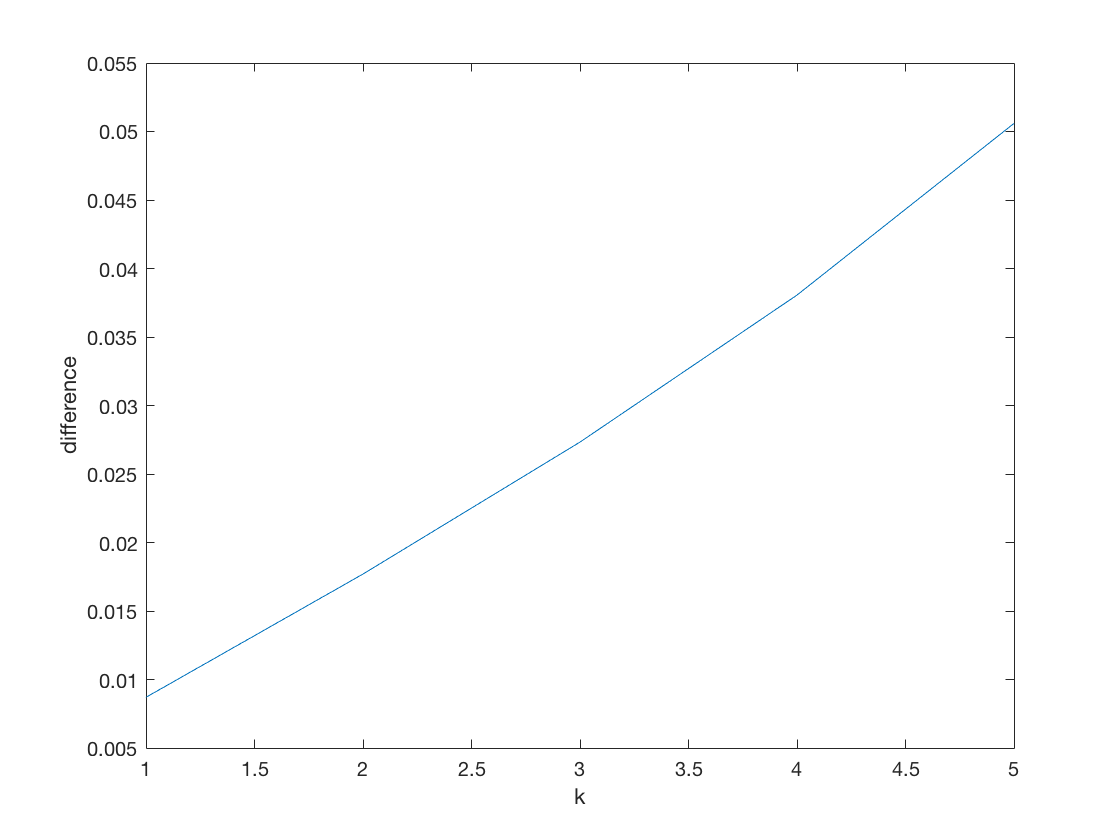
\includegraphics[scale=0.4]{e321.png}
When choosing 101 sampling points, the difference between $b_{k}$ and $-2\times Imag(c_{k})$ is\\ 
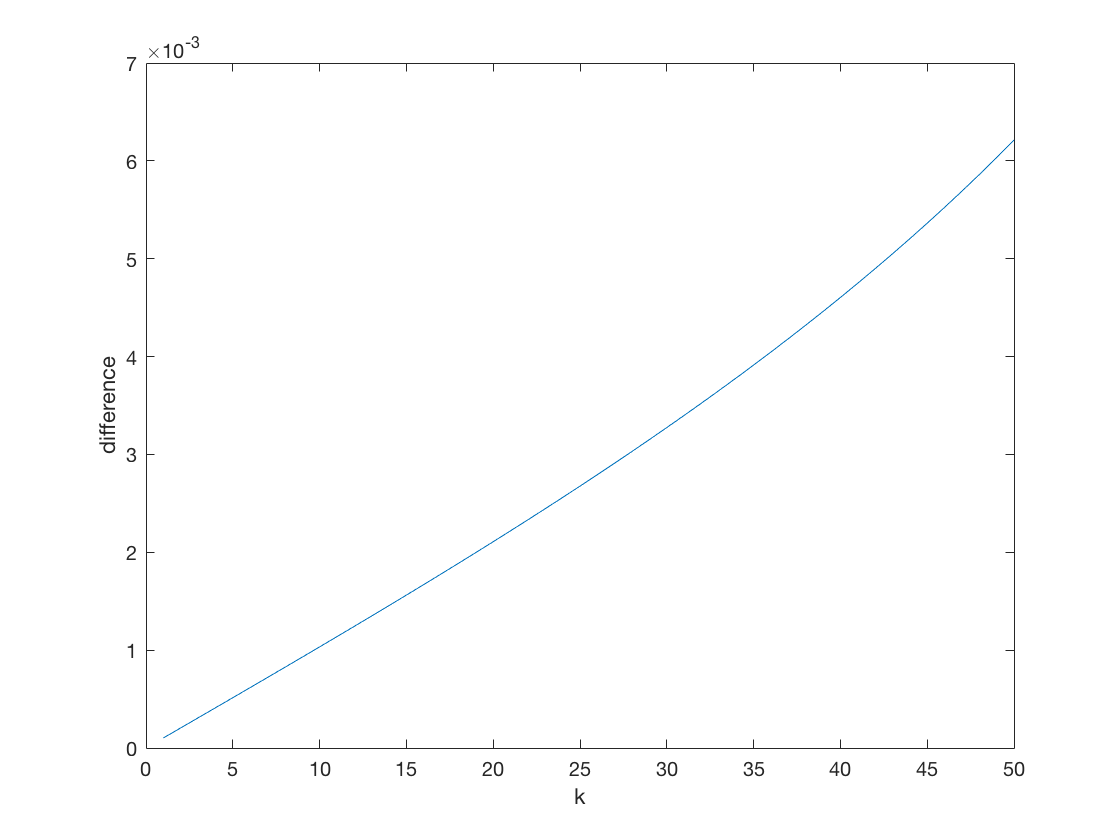
\includegraphics[scale=0.4]{e322.png}
When choosing 1001 sampling points, the difference between $b_{k}$ and $-2\times Imag(c_{k})$ is\\ 
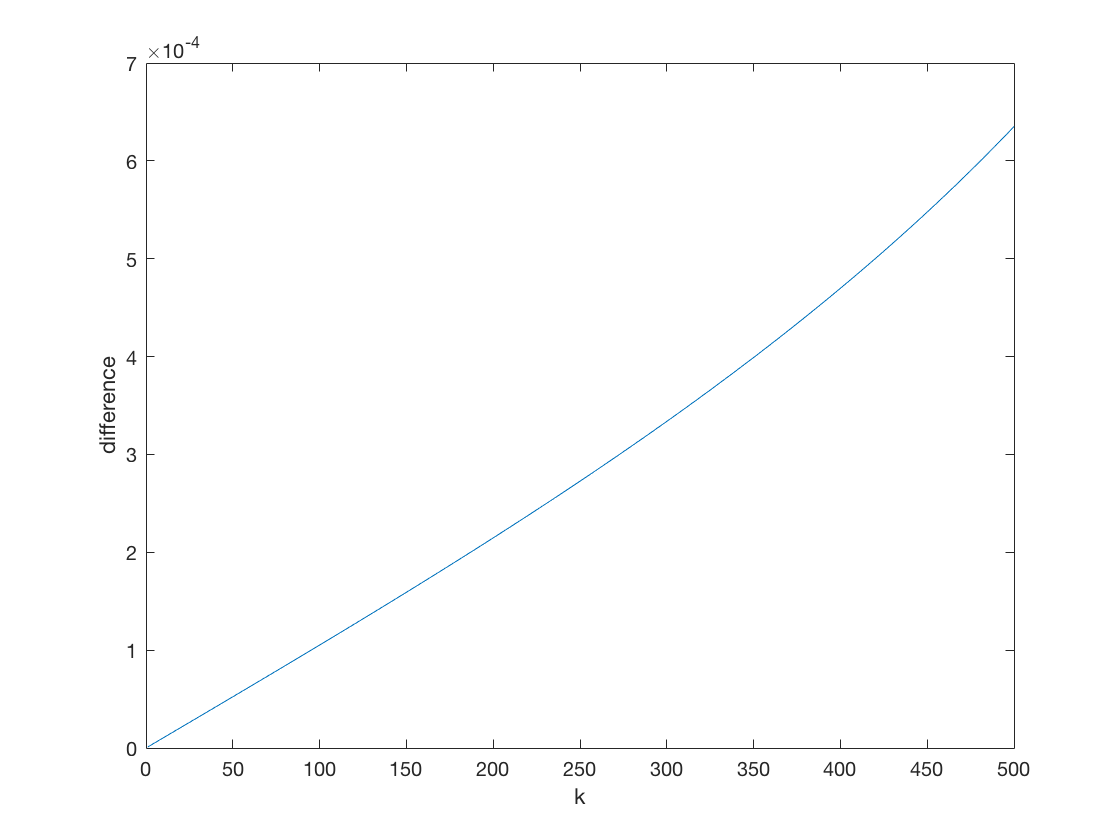
\includegraphics[scale=0.4]{e323.png}\\
As we can see here, the difference decrease really fast as we have more and more sampling points.
\section{Exercise 4}
%When the function is periodic on $[a,b]$ instead of being periodic on the interval of $[0,1]$\\\\
%\centerline{Let $I = b-a$, then $C_{k} = \sum_{0}^{n-1}f(x_{n})e^{-2\pi i \frac{k}{I}x_{n}}$}\\\\
%When approximating the original function, we have \\\\
%\centerline{$f(x)$ = $\frac{a_{0}}{2}+\sum_{0}^{n-1}2Real(C_{k})cos(\frac{2\pi}{I}kx)-2Imag(C_{k})sin(\frac{2\pi}{I}kx)$}\\\\
%For example,\\\\
%\centerline{Let $f(x) = x-5$ on interval $[5,10]$}\\\\
Here we introduce a mapping from interval [0,1] to [a,b]\\\\
\centerline{$t = (b-a)x+a$, where $x$ $\in$ [0,1], t $\in$ [a,b]}\\\\
Let's call this mapping t(x), and the inverse mapping x(t). \\\\
\centerline{$x = \frac{t-a}{b-a}$}\\\\
We use the points on [0,1] when calculating the coefficients,\\\\ 
\centerline{Then $C_{k} = \sum_{0}^{n-1}f(t_{n})e^{-2\pi i k x(t_{n})}$}\\\\
When approximating the original function, we have\\\\
\centerline{$f(x) = \frac{a_{0}}{2}+\sum_{k=1}^{\infty}a_{k}cos(2\pi k x(t))+b_{k}sin(2\pi k x(t))$}\\\\
For example, let f(x) = x, we set the interval to be [2,9], when having 101 sampling the points, the graph is the following:\\\\
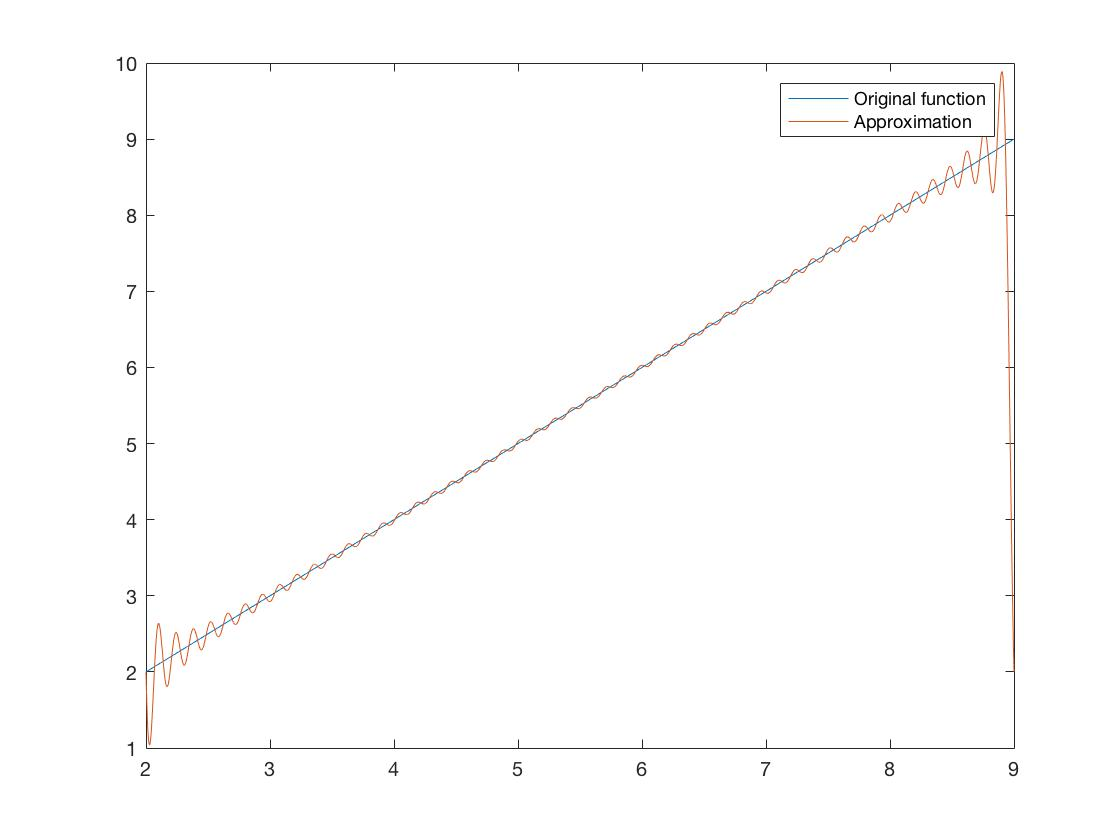
\includegraphics[scale=0.3]{e41.jpg}
\section{Exercise 5}
Let's take $f(x) = x^{\frac{3}{2}}$ as an example, this function is 1 time differentiable, the reason is the following, for its second derivative $f''(x) = \frac{3}{4}x^{-\frac{1}{2}}$ , it doesn't exist at x=0. Following this pattern, we can find a series of k times differentiable functions. For example, functions that have the form\\\\
\centerline{$f(x) = Cx^{\frac{1}{2}+k}$, where C is a constant}\\\\
are k times differentiable.\\\\
Take $f(x) =x^{\frac{1}{2}+2}$ which is a 2 times differentiable function, the error is plotted in the following graph:\\\\
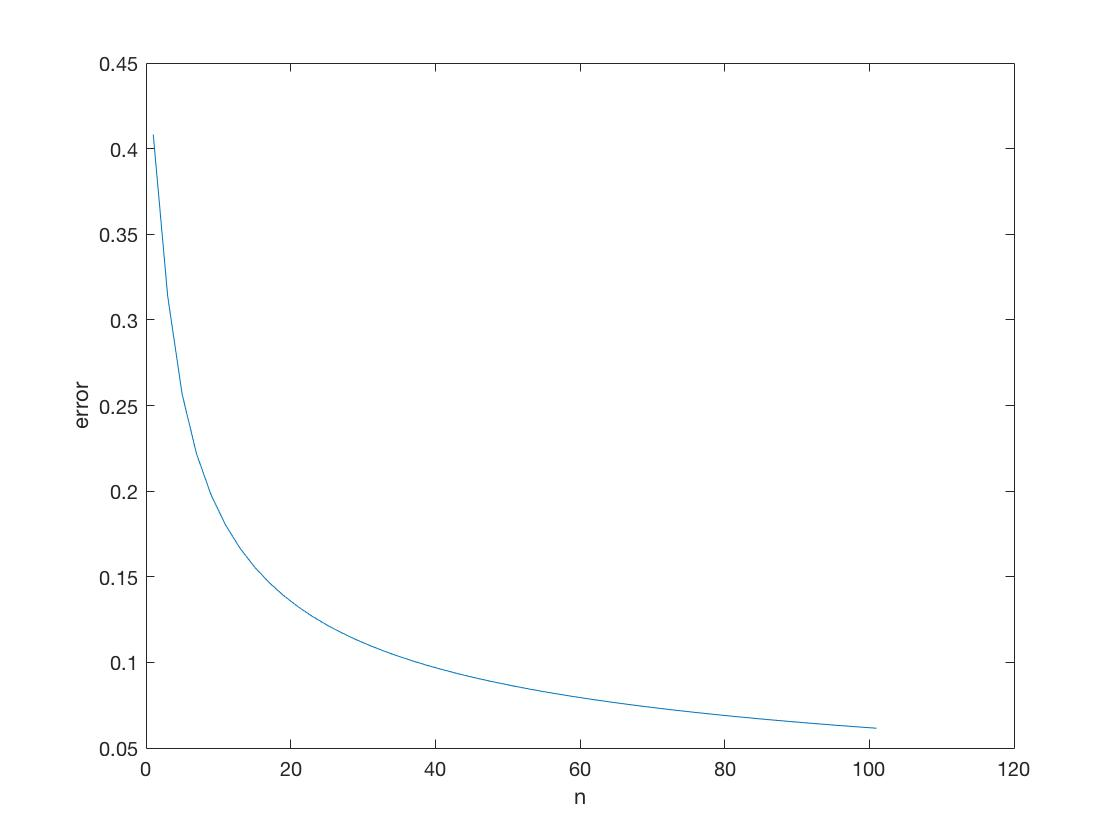
\includegraphics[scale=0.3]{e51.jpg}

\section{Exercise 6}
\subsection{8.1}
The phone number is \\\\
\centerline{15086477001}\\\\
The frequency plots of every single digit are the following(Read from left to right and from top to bottom):\\\\
\begin{center}
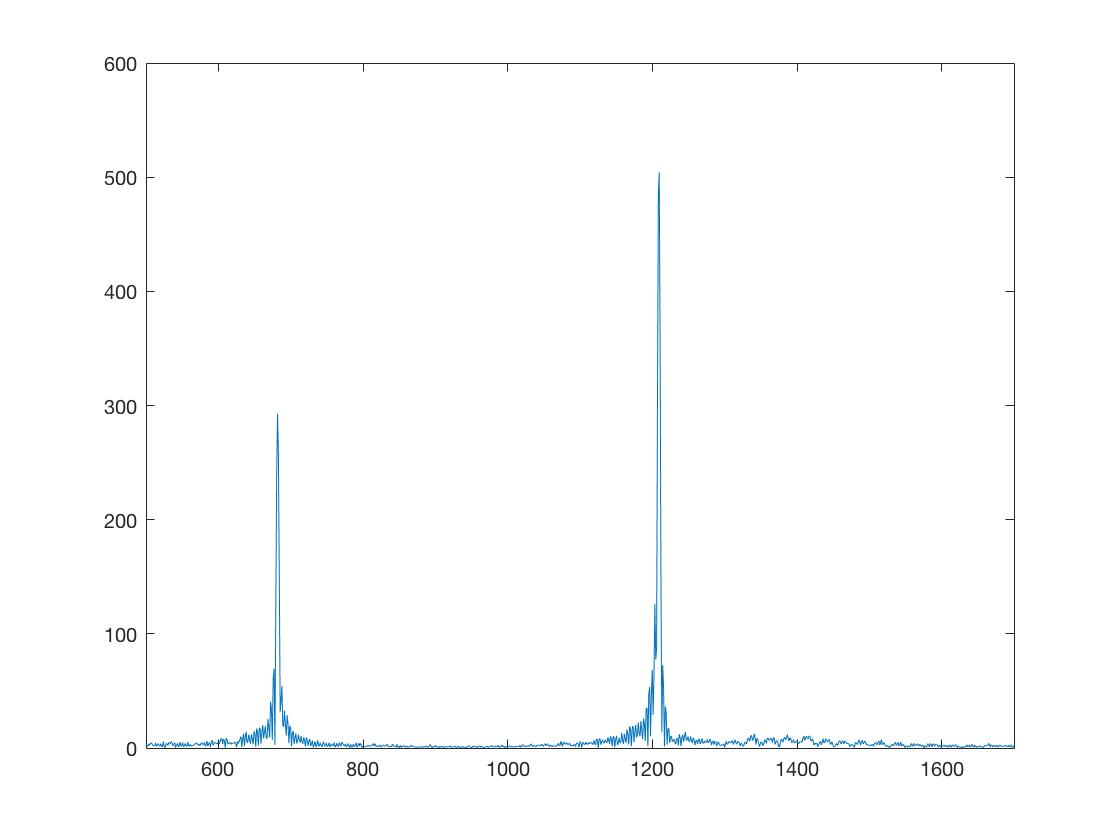
\includegraphics[width=.3\textwidth]{e60.jpg}
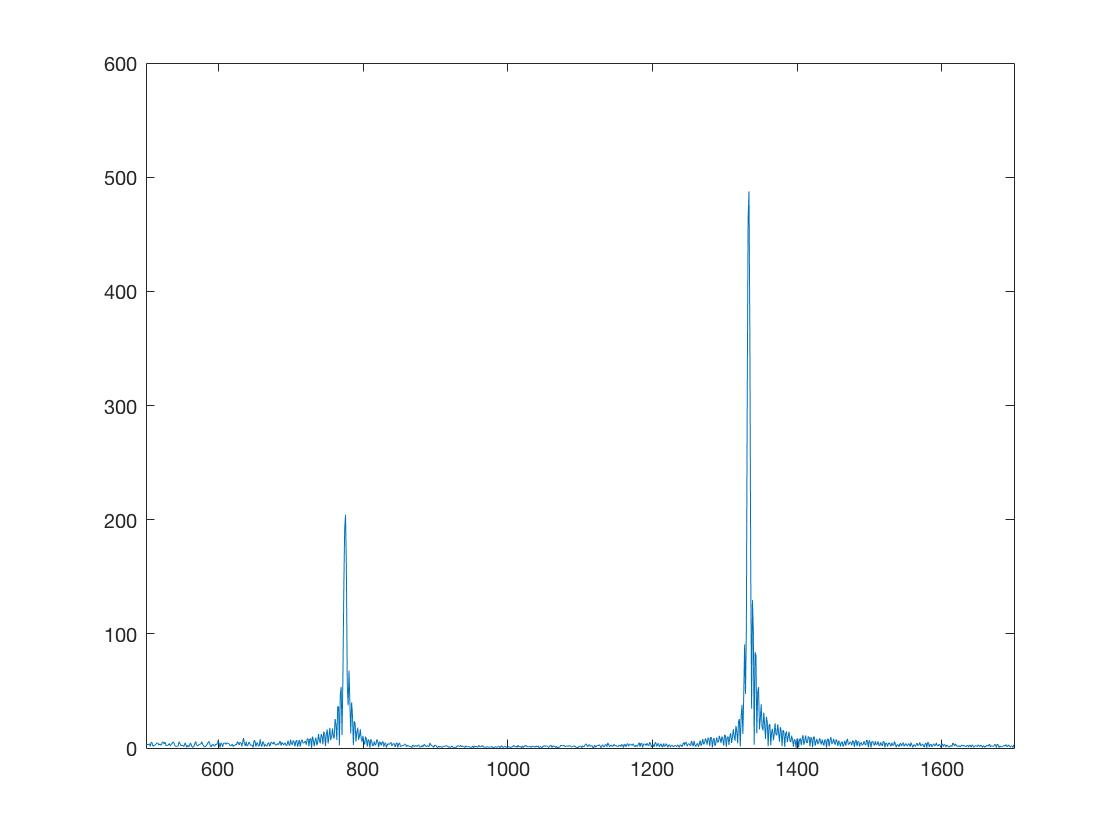
\includegraphics[width=.3\textwidth]{e61.jpg}
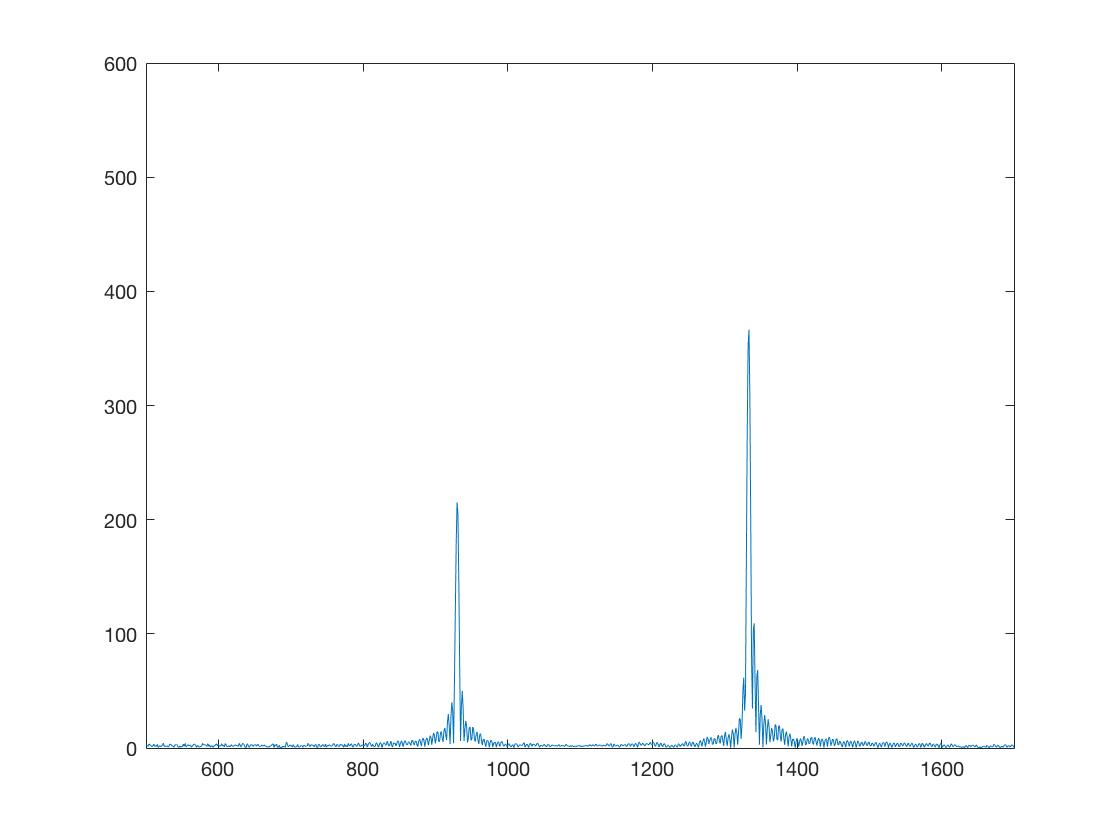
\includegraphics[width=.3\textwidth]{e62.jpg}
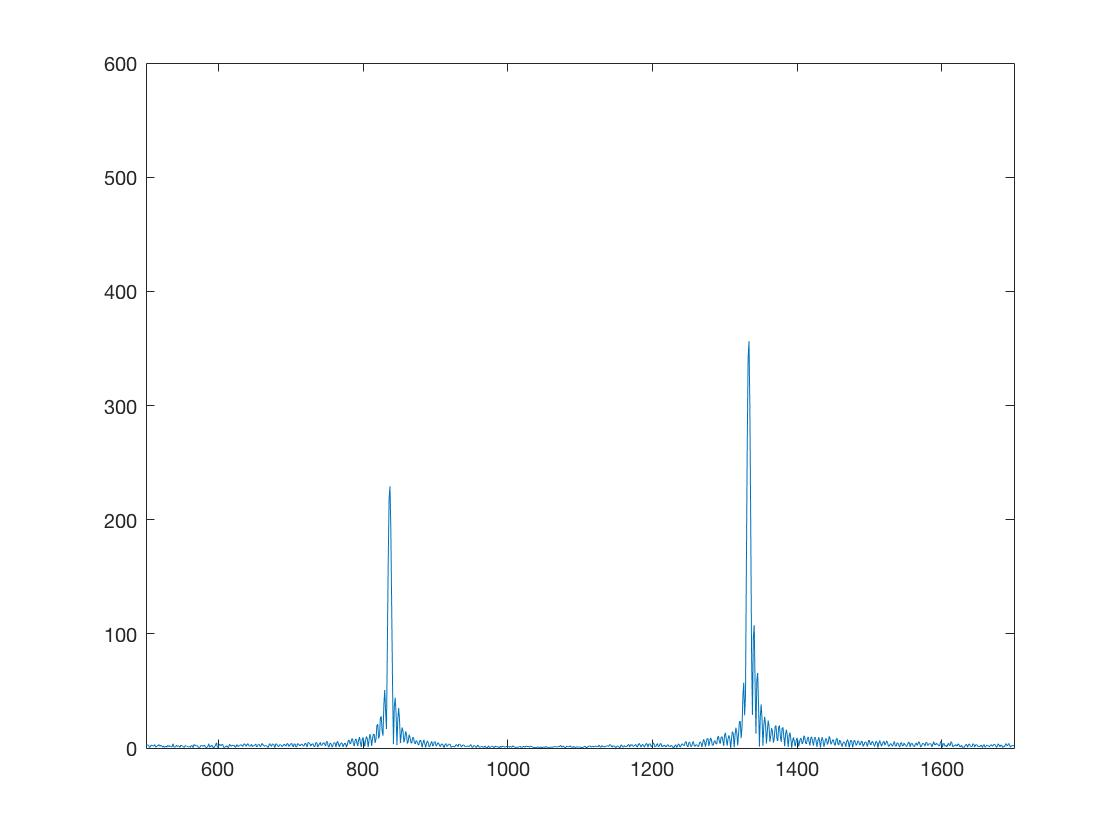
\includegraphics[width=.3\textwidth]{e63.jpg}
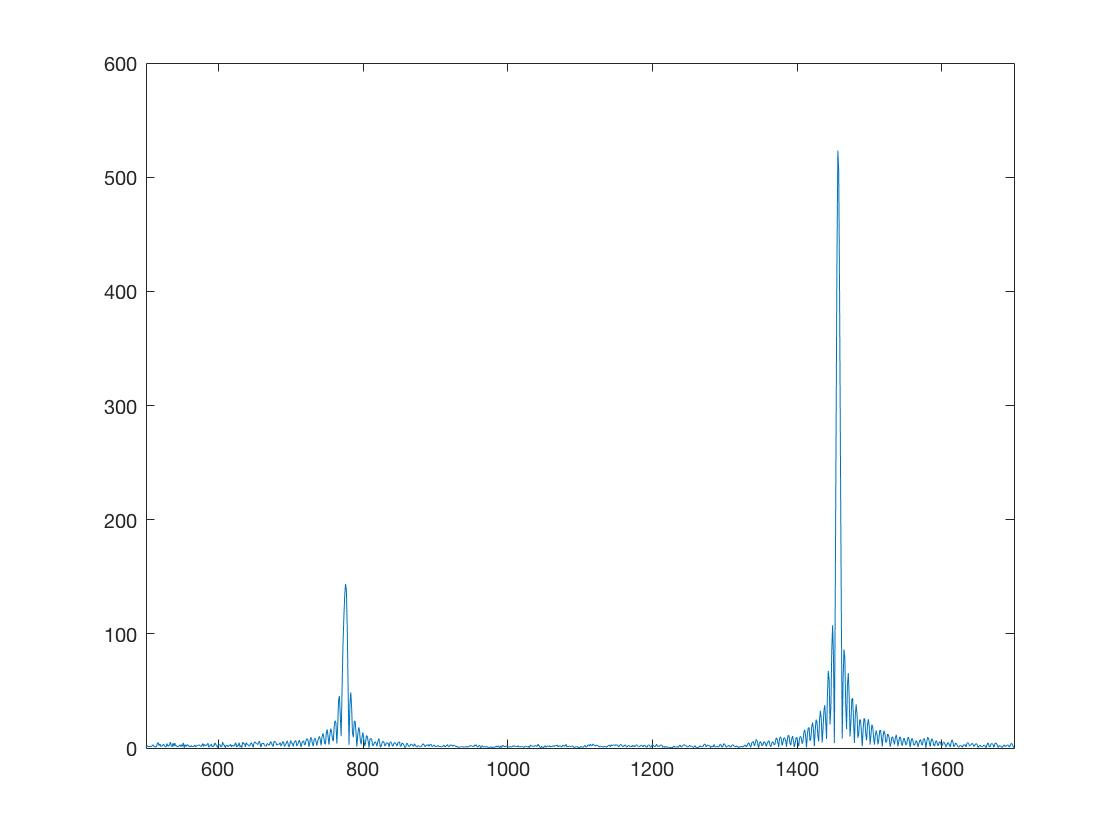
\includegraphics[width=.3\textwidth]{e64.jpg}
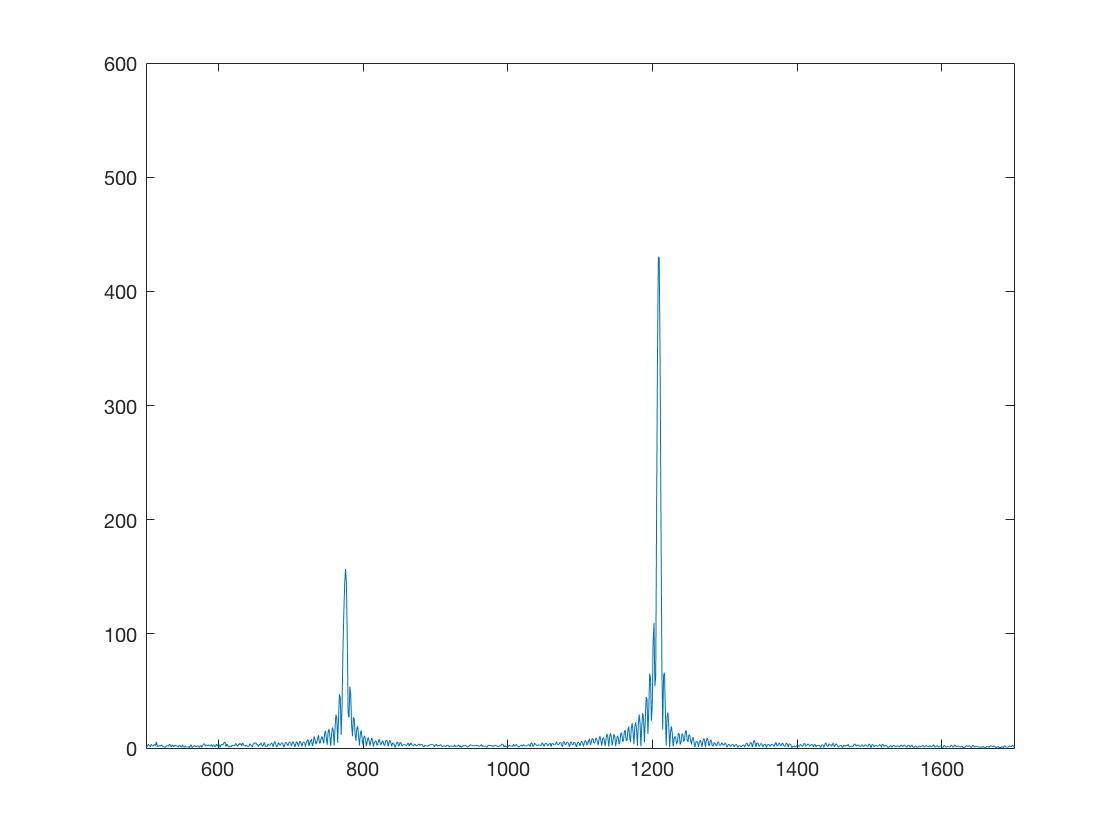
\includegraphics[width=.3\textwidth]{e65.jpg}
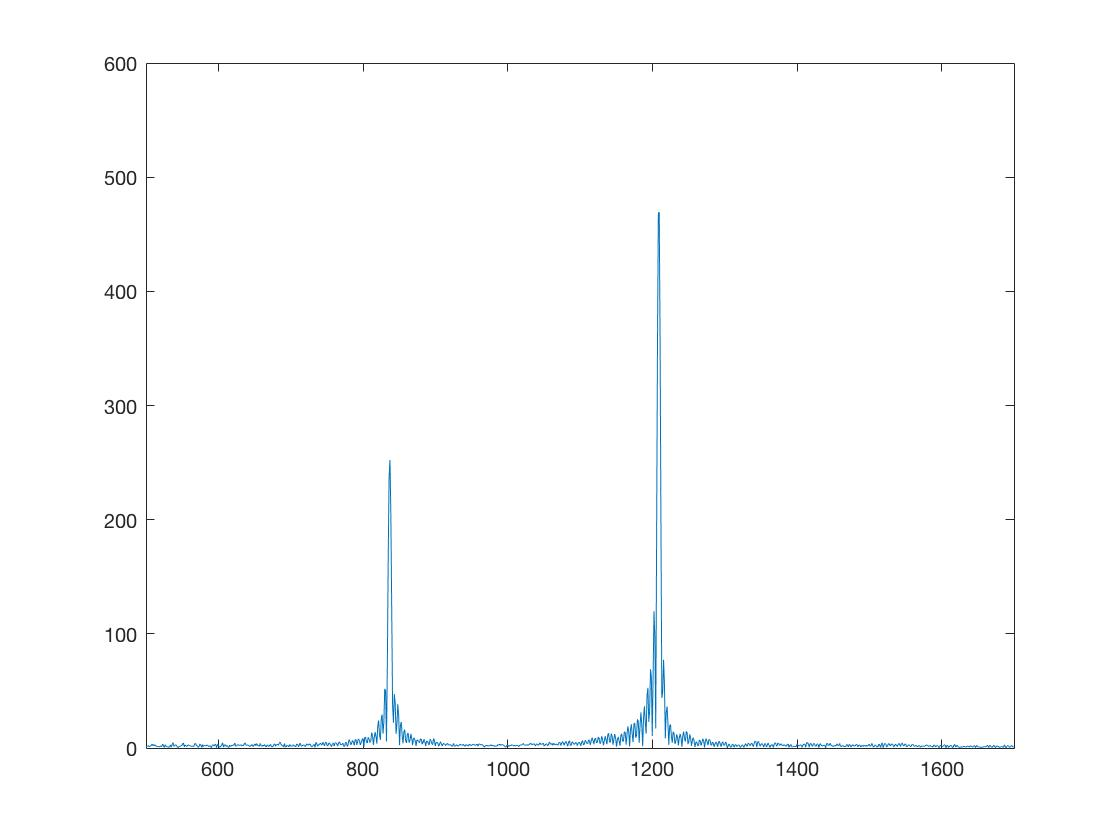
\includegraphics[width=.3\textwidth]{e66.jpg}
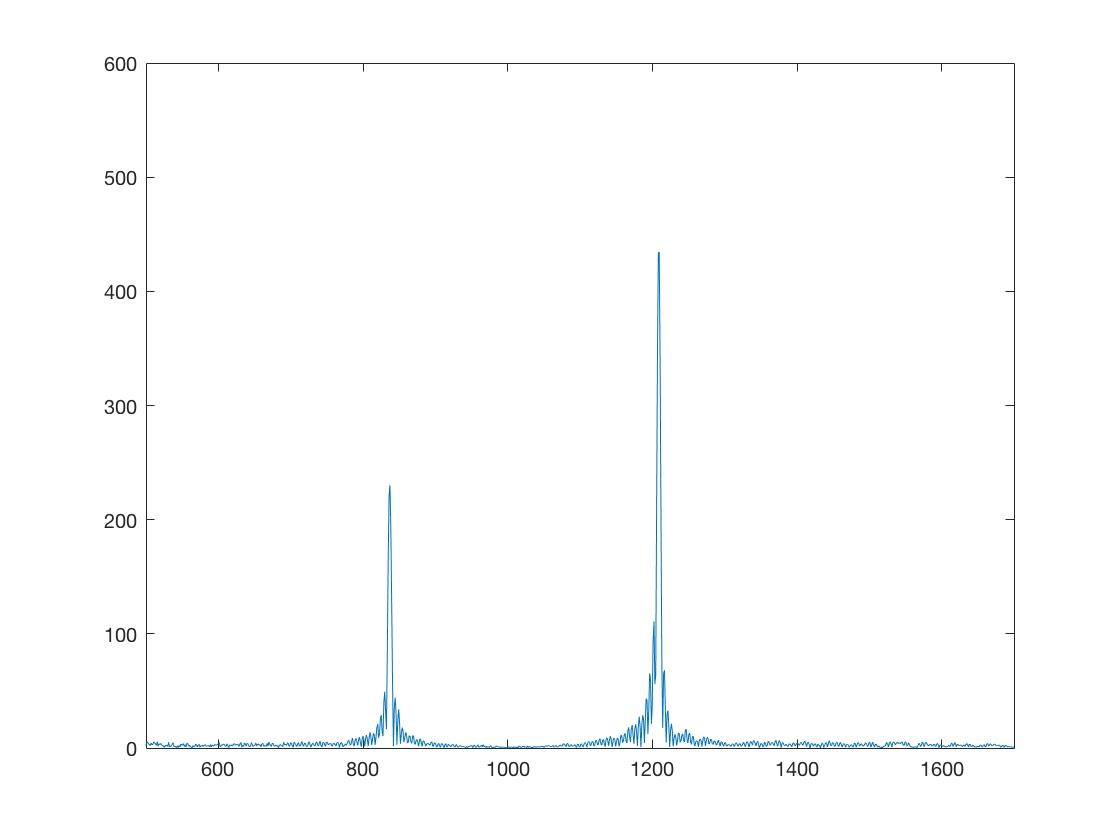
\includegraphics[width=.3\textwidth]{e67.jpg}
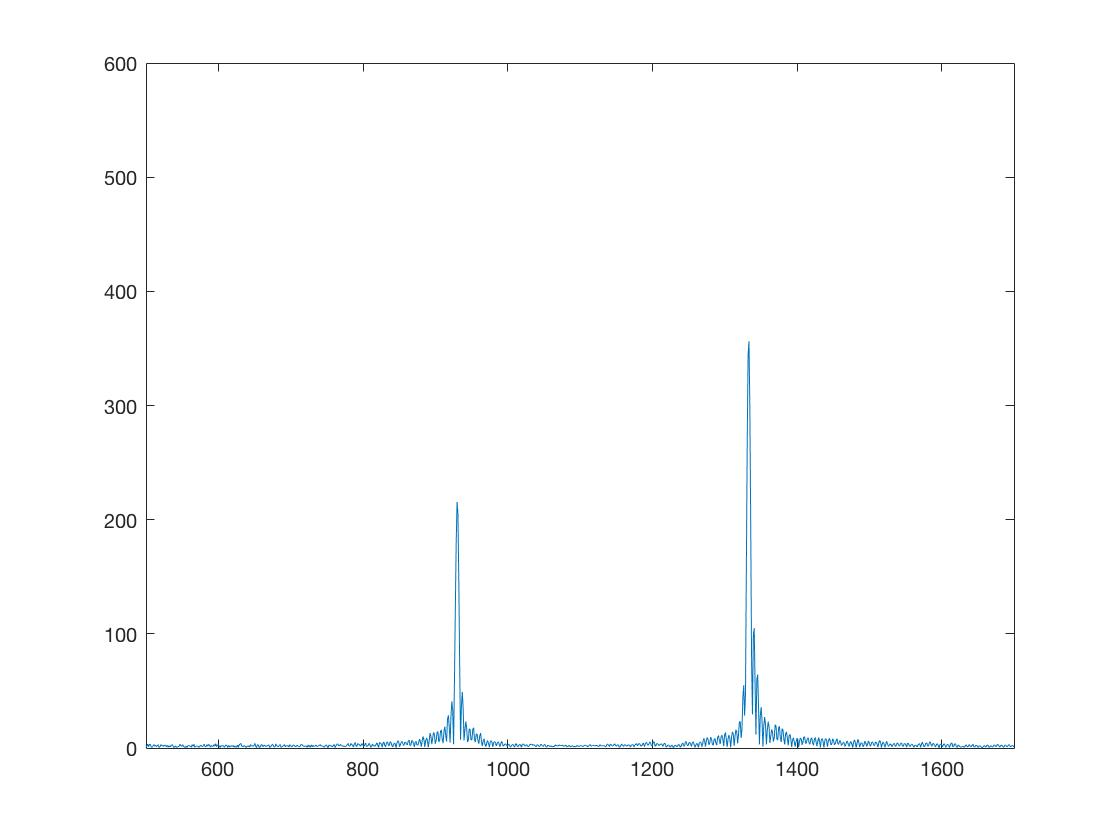
\includegraphics[width=.3\textwidth]{e68.jpg}
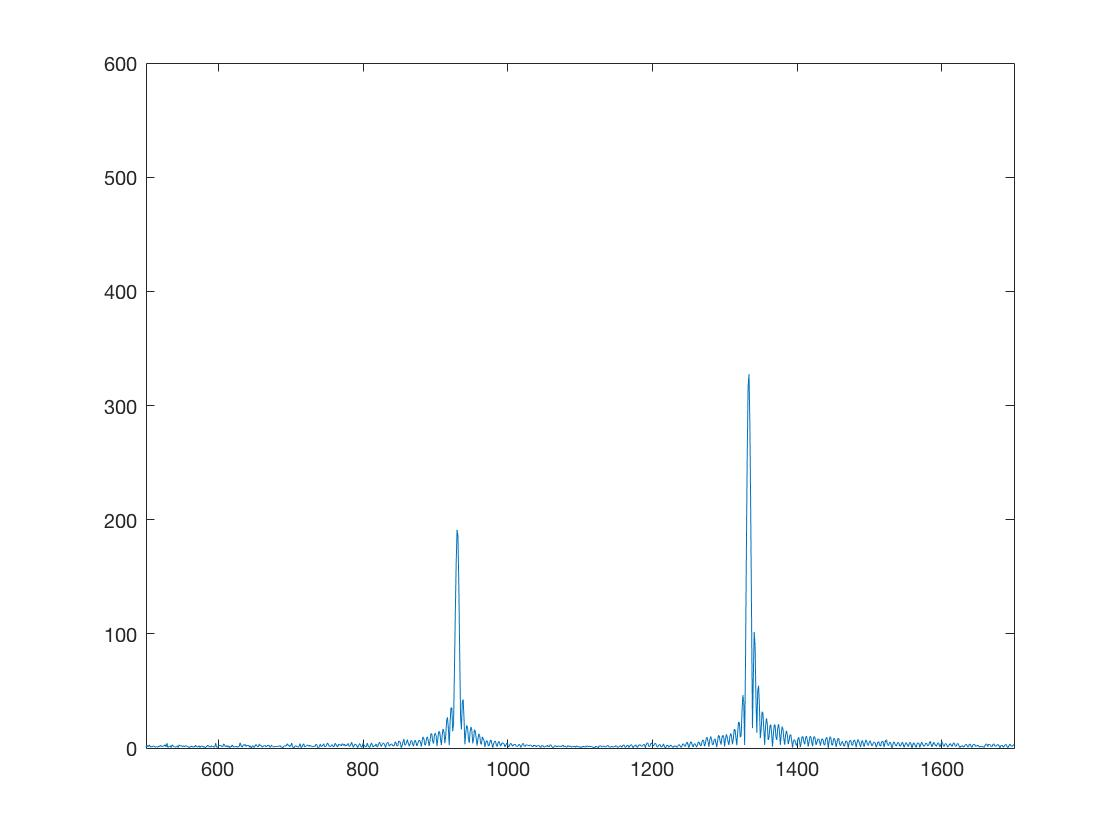
\includegraphics[width=.3\textwidth]{e69.jpg}
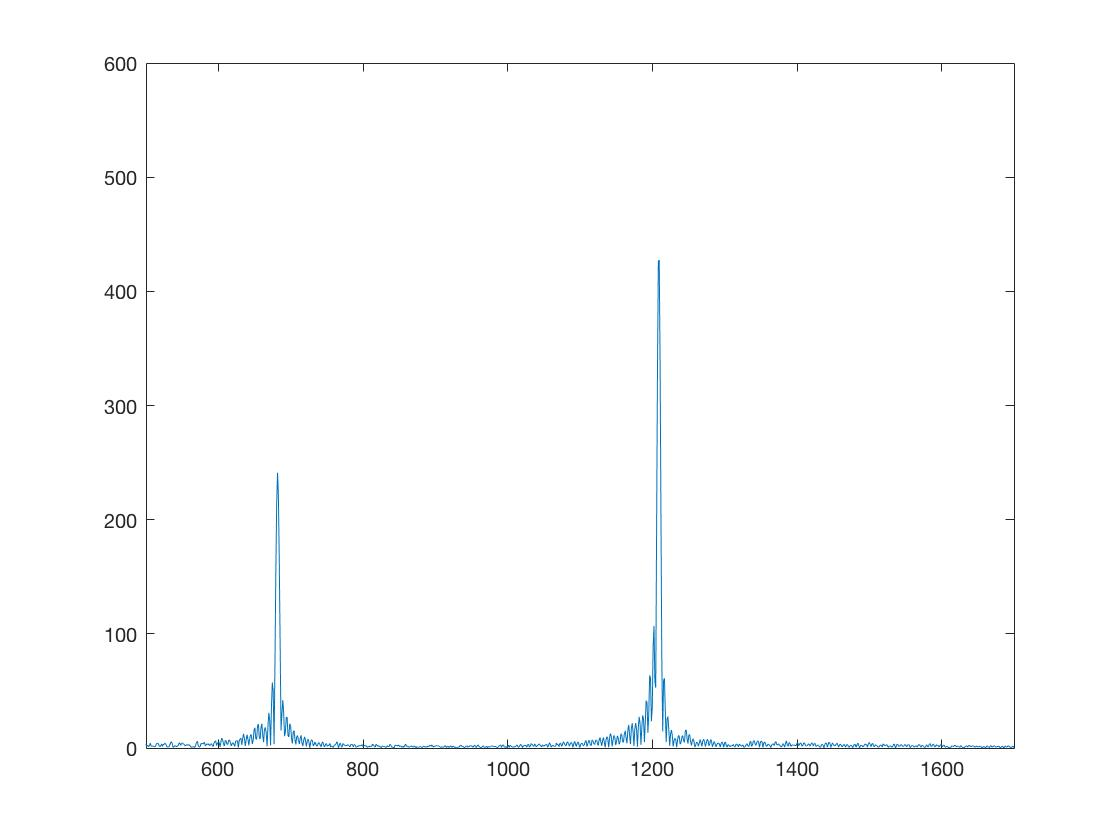
\includegraphics[width=.3\textwidth]{e10.jpg}
\end{center}
\subsection{8.2}
Dear TA, trust me, my code works, I have tested it on different numbers.\\
The only below only shows the added part to the function, this piece of code is added to the end of the function.
\begin{lstlisting}[language=Octave, basicstyle=\ttfamily]
else
    len = length(arg);
    fr = [697 770 852 941];
    fc = [1209 1336 1477];
    Fs = 32768;
    t = 0:1/Fs:0.25;
    for i = 1:1:len
        c = arg(i);
        if c == '-'
            continue
        else
            switch c
                case '*'
                    k = 4; 
                    j = 1;
                case '0'
                    k = 4; j = 2;
                case '#'
                    k = 4; 
                    j = 3;
                otherwise
                    d = c-'0'; 
                    j = mod(d-1,3)+1; 
                    k = (d-j)/3+1;
            end
            y1 = sin(2*pi*fr(k)*t);
            y2 = sin(2*pi*fc(j)*t);
            y = (y1 + y2)/2;
            sound(y,Fs)
            pause(0.4)
        end
    end
end

\end{lstlisting}

\end{document}
